\chapter{Background}
% First list what is going to be done in this chapter (outline)
In this section, we will review the relevant concepts and technologies that are necessary to understand the rest of the work. The topics are organized in two sections, Cyber Threat Intelligence Sharing and Dataspaces. The former will discuss the current state of the CTI sharing, its goals, and it challenges. The latter will analyse data spaces, its context and what it promises. Our goal is set the stage for our later discussions on how the data spaces could facilitate CTI sharing. 

\section{Cyber Threat Intelligence Sharing}
% In this section we will present the concept of \gls{cti} in more detail to understand why is it important, what are the 

\subsection{Overview of Cyber Threat Intelligence}

\subsubsection{Intelligence}
We start with the term intelligence. 
Intelligence is often is associated with a state defense, an example intelligence organization is the Central Intelligence Agency (CIA). 
However, it could be relevant in the private sector as well. 
A relevant concept here is the Competitive Intelligence which is about gaining marketplace competitiveness through researching the market rivals. The intelligence definition that we will use throughout this thesis is the following:

\smallskip
The process and the product of the process of collecting, analysing and disseminating the information which is helpful in decision making.

To ensure the effectiveness, a systematic approach to intelligence is necessary. Therefore a lifecycle is often mentioned in the litereture to explain all the stages in the process. It consists of 6 stages that follow each other in circle, where each one builds on the previous one (Figure \ref{fig:cti-lifecycle}).

\begin{figure}[ht]
    \centering
    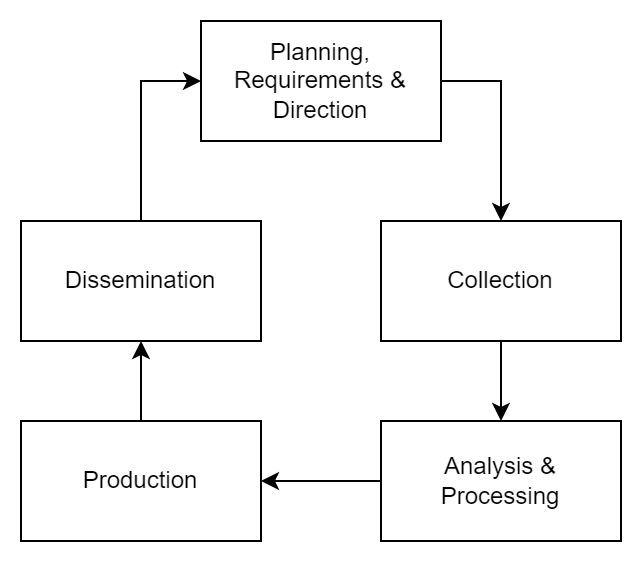
\includegraphics[width=0.5\textwidth]{diagrams/background/intelligence-cycle.png}
    \caption{The Intelligence Cycle \cite{lee_cyber_2023}}
    \label{fig:cti-lifecycle}
\end{figure}

\subsubsection{Cyber Threat Intelligence}
% Why CTI and why (already in motivation?)
By applying the provided definition of intelligence to the context of cyber security we could define Cyber threat intelligence (CTI) as follows:

\smallskip
The process of collecting, analyzing, and disseminating information about potential or current cyber threats. 

CTI is an important part of the security posture of any organization, because a constant study of cyber threats is necessary to mitigate and prevent cyber incidents.
It is due to the increase in the attack surface following the digitalization and emergence of new attack vectors developed by the threat actors, hence a constant evolution of the threat landscape.

\subsubsection{Cyber Threat Information Types}
CTI relies on collecting data from diverse sources, including security tools, threat feeds, honeypots, forums, social media platforms, and other relevant online and offline sources. 

\subsubsection{Types of CTI}
CTI could be categorized into three different types:

\paragraph{Strategic CTI -- Why?}
Strategic CTI expresses high level insights such as overall threat landscape, the motivations of threat actors, and the business or political impact of the threats. It mainly benefits executive management and other decision making departments by allowing data driven decision making to reduce the risks of cyber attacks.

\paragraph{Tactical CTI -- How?}
Tactical CTI is about "how" the threats can cause incidents. Examples are the tactics, techniques, and procedures (TTPs) used by threat actors, vulnerabilities in the organization's security infrastructure, and the strategies that were used to mitigate the impact of the breach. Security teams can achieve more efficiancy by not repeating the work already done leading to more agile cyber incident response.

\paragraph*{Technical CTI -- What?}
Technical CTI concerns with the indicators of compromise, meaning concrete technological signs about the attacker or an attack, such as malware hashes or malicious IP addresses. Another term for these products is the Indicator of Compromise (IoC), which refer to any technical observable showing an undergoing attack. Security teams and system administrators can feed IoCs to the firewalls and intrusion prevention systems (IPSs).

\subsection{Benefits of Collaborative CTI}
The are four categories of benefits identified in \cite{zibak_cyber_2019}. First, the operational benefits include reduce duplicate information handling and support breach detection and response. Second, organisational benefits such as improving overall security posture and situational awareness, combating skills gap, cross-checking different sources, and expanding professional networks. Third, economic benefits which are total cost savings, allowing governmental subsidies, reducing investment uncertainties. Lastly, policy related benefits such as reinforcing the connection with the government agencies.

\subsection{Current State of Cyber Threat Intelligence}
TODO: outline

\subsubsection{Automation and Standardization}
There are various channels for CTI exchange. \cite{wagner_cyber_2019} mentions meetings, E-mails and phonecalls, shared databases, web portals or data feeds. Currently sharing CTI requires a lot of manual labor not only on the provider side, to prepare the information, but also on the consumer side to analyze the quality and relevance of the data \cite{wagner_cyber_2019}. Automated CTI exchange is not expected in the near future to drop the security analyst from the loop completely, but it tries to speed up the whole process \cite{wagner_cyber_2019}. To enable expressing CTI in a machine readable format, some protocols have been defined  (Table \ref{tab:cti-protocols})

\begin{table}[ht]
    \label{tab:cti-protocols}
    \centering
    \begin{tabular}{|p{0.5\textwidth} p{0.5\textwidth}|}
    \hline
    \textbf{Title} & \textbf{Description} \\
    \hline
    \hline
    Structured Threat Information eXpression (STIX) \cite{stix_documentation_2024} & Structured language for CTI sharing (human and machine readable in JSON) \\
    \hline
    Trusted Automated eXchange of Indicator Information (TAXII) \cite{stix_documentation_2024} & Language to share CTI (open transport mechanism with native support for HTTP and HTTPS) \\
    \hline
    Malware Attribution Enumeration and Characterization (MAEC) \cite{maec_project_documentation_2024} & A standardized langauge for sharing structured information about malware (human and machine readable in XML) \\
    \hline
    Incident Object Description Exchange Format (IODEF) \cite{kampanakis_incident_2017} & Framework for sharing computer security incidents in XML \\
    \hline
    Vocabulary for Event Recoding and Incident Sharing (VERIS) \cite{veris_framework} & Language to describe structured security events \\
    \hline
    \end{tabular}
    \caption{CTI Protocols \cite{wagner_cyber_2019}}
\end{table}

\subsubsection{Current Sharing Models and Platforms}

As shown in \ref{fig:sharing-models}, there are three types of sharing. First, peer to peer, which is a direct exchange, second, peer to repository which allow for subscription to published events, and third, a hybrid model that incorporates the mentioned models.

\begin{figure}[ht]
    \centering
    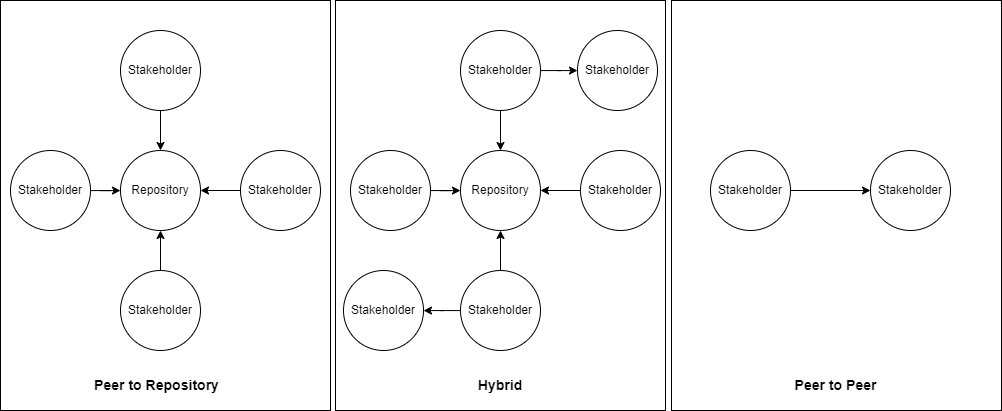
\includegraphics[width=\textwidth]{diagrams/background/sharing_models.png}
    \caption{Information Sharing Models \cite{wagner_cyber_2019}}
    \label{fig:sharing-models}
\end{figure}

The repository model often happen in a community of participants with shared goals where they know and trust each other by means of meetings and so on. An example type of existing sharing communities are Information Sharing and Analysis Centers (ISACs). These are non-profit organizations that help organizations in a specific sector, usually a critical national infrastructure, e.g. electricity, water, gas, health care, finance, etc., to share CTI with each other. 

\paragraph{EE-ISAC}
An example ISAC would be European Energy Information Sharing and Analysis Center (EE-ISAC) which has acquired over 30 members from utilities, academia, governmental and non-governmental organizations since its foundation in 2015. Members exchange cyber threat information through plenary meetings, working groups, and a dedicated platform (based on MISP). 
The information exchange is based on a trust achieved by confidentiality agreements and regular physical meetings with the same members. 
\cite{wallis_ee-isacpractical_2022}

There are also some CTI that are accessible via internet, these are called Open Source Intelligence (OSINT), public CTI feeds or social media (e.g. Twitter) security channels are examples.

Another approach to accomplish a CTI repository is through Threat Intelligence Platforms (TIPs). These platforms not only allow sharing CTI between users but also allow collection from various sources (e.g. OSINT, 3rd party intelligence) and integration to interanal security systems such as Firewall, Intrusion Prevention Systems (IPSs), and Security Information and Event Management (SIEM) \ref{fig:tip}. A list of available TIPs are in mentioned in table \ref{tab:tips}

\begin{figure}[ht]
    \centering
    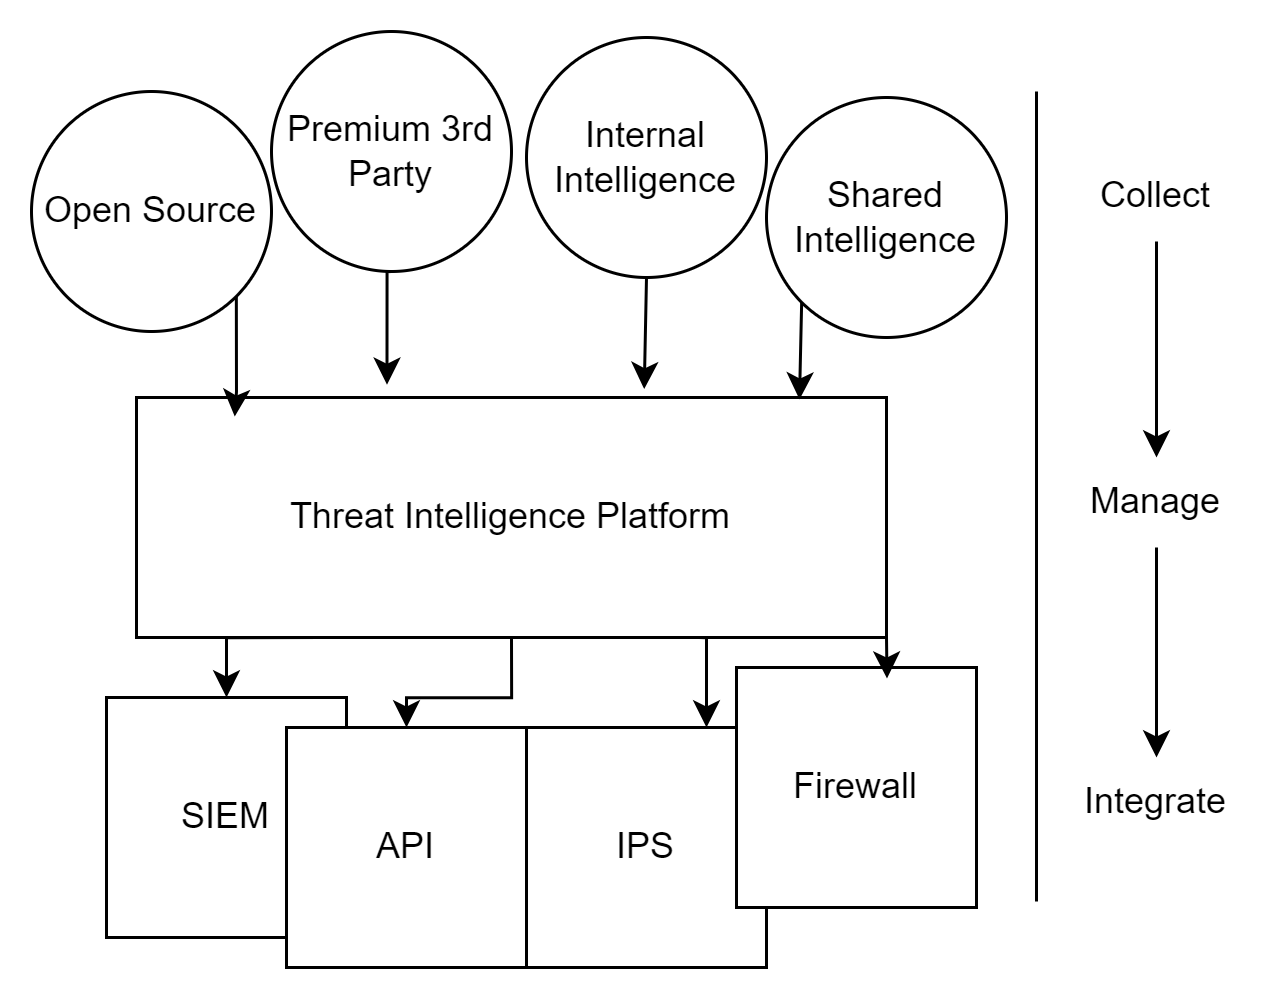
\includegraphics[width=\textwidth]{diagrams/background/threat-intelligence-platform.png}
    \caption{Threat Intelligence Platform (TIP) \cite{anomali_tip_2024}}
    \label{fig:tip}
\end{figure}

\begin{table}[ht]
    \centering
    \label{tab:tips}
    \begin{minipage}{\textwidth}
        \begin{tabular}{l c c}
            \textbf{TIP} & \textbf{Paid} & \textbf{Open Source} \\
            \hline
            Malware Information Sharing Platform (MISP) \footnote{https://www.misp-project.org} & & \checkmark \\
            Anomali ThreatStream \footnote{https://www.anomali.com/products/threatstream} & \checkmark & \\
            ThreatConnect \footnote{https://threatconnect.com} & \checkmark & \\
            ThreatQ \footnote{https://www.threatq.com/} & \checkmark & \\
            EclecticIQ Platform \footnote{https://www.eclecticiq.com/} & \checkmark & \\
            OpenCTI \footnote{https://filigran.io/solutions/products/opencti-threat-intelligence/} & \checkmark & \checkmark \\
            IBM X-Force Exchange \footnote{https://exchange.xforce.ibmcloud.com/} & & \\
            AlienVault Open Threat Exchange (OTX) \footnote{https://otx.alienvault.com/} & & \\
            CrowdStrike \footnote{https://www.crowdstrike.com/} & \checkmark & \\
            \hline
        \end{tabular}
    \end{minipage}
    \caption{Threat Intelligence Platforms}
\end{table}

\subsubsection{Regulations and Recommendations}
The landscape of Cyber Threat Intelligence (CTI) sharing is heavily influenced by a complex web of regulations and recommendations. Two important regulations are General Data Protection Regulation (GDPR) and The Network and Information Systems (NIS) Directive. 

\paragraph{GDPR} aims to protect the personal data and privacy of individuals within the EU and addresses the transfer of personal data outside the EU. GDPR is highly relevant in the context of CTI due to the potential inclusion of personal data in the threat intelligence information, such as IP addresses, email addresses, and other identifying information. 

\paragraph{NIS} directive aims at improving the overall level of cybersecurity across the EU. It mandates the EU states to establish a national Computer Security Response Teams (CSIRTs) to monitor, detect, and respond to cyber incidents. These CSIRTs are required to collect information from private sector and share this with other national CSIRTs. It recommends the globally accepted standards and best practices for CTI sharing, such as the STIX/TAXII protocols.

Apart from the regulations, there are also recommendations from standardization bodies that try to harmonize the CTI sharing. Three of the most important standardization efforts are from European Union Agency for Cybersecurity (ENISA), International Organization for Standardization (ISO), and National Institute of Standards and Technology (NIST).

The first one is the ENISA's "Proactive Detection Of Network Security Incidents" which aims to enhance the capabilities of CERTs in detecting network security incidents by utilizing both external information sources and internal monitoring tools. This report provides guidelines and best practices to proactively identify and respond to potential cyber threats, thus improving the overall cybersecurity posture within the European Union.
The second one is the ISO's "Information technology -- Security techniques -- information security management for intersector and inter-organizational communications", which offers a standardized framework for managing and protecting sensitive information across different sectors and organizations. This standard ensures that information security measures are consistently applied, enabling secure and effective communication and collaboration between entities.
The third one is the NIST's "Guide to Cyber Threat Information Sharing" which provides guidelines and best practices for sharing cyber threat information among organizations. This guide aims to enhance situational awareness and improve the collective defense against cyber threats by facilitating timely and actionable information exchange. It outlines the processes, policies, and technical aspects of effective cyber threat information sharing to help organizations mitigate risks and respond to incidents more efficiently.

The aspects that are addressed in each one is summarized in table \ref*{tab:standardization}. 

\begin{table}[ht]
    \centering
    \begin{tabular}{ | l | c c c | }
    \hline
    \textbf{Aspect} & \textbf{ENISA} & \textbf{ISO} & \textbf{NIST} \\ \hline
    Protection of shared information & \checkmark & \checkmark & \\
    Cyber security risk management &  & \checkmark & \\
    Privacy preservation in information sharing & \checkmark &  & \\
    Data format, protocols and standards &  &  & \checkmark \\
    Data quality improvement & \checkmark &  & \\
    Incident handling process & \checkmark & \checkmark & \\ 
    \hline
    \end{tabular}
    \caption{Aspects addressed by the different standardization efforts \cite{skopik_survey_2016}.}
    \label{tab:standardization}
\end{table}

\subsection{Challenges of CTI Sharing}
Despite the benefits of CTI sharing, there are several challenges that hinder the effective sharing of cyber threat intelligence. \cite{johnson_guide_2016} lists the following general challenges: Establishing Trust, Achieving Interoperability and Automation, Safeguarding Sensitive Information, protecting classified information, enabaling infromation consumption and publication. \cite{johnson_guide_2016} also mentions some challenges that are specific to the consumer side: infrustracture for accessing external information, evaluation of the quality of the information. These challenges are summarized in table \ref{table:barriers}.

\begin{table}[ht]
    \centering
    \begin{tabular}{| m{6cm} | m{3cm} | m{3cm} |}
    \hline
    \textbf{Name} & \textbf{Involved Actor} & \textbf{Category} \\
    \hline
    Achieving Interoperability and Automation & Both & Operational \\
    \hline
    Evaluating the Quality of Received Information & Consumer & Operational \\
    \hline
    Safeguarding Sensitive Information (PII, Organization Secrets, Classified Information) & Both & Regulatory \& Operational \\
    \hline
    Establishing Trust & Both & Organizational \\
    \hline
    Free Riding Effect & Both & Economical \\
    \hline
    Risk of Reputation Loss & Provider & Economical \\
    \hline
    Enabling Information Consumption and Publication (Infrastructure for automatic sharing of indicators) & Both & Technical \\
    \hline
    Accessing External Information (Infrastructure) & Consumer & Technical \\
    \hline
    \end{tabular}
    \caption{Barriers in Cyber Threat Information Sharing. Adopted from various sources \cite{johnson_guide_2016}, \cite{zibak_cyber_2019}.}
    \label{table:barriers}
\end{table}

\subsubsection{Conclusion}
Cyber Threat Intelligence (CTI) is a young field that is rapidly evolving. In this section, we have discussed this concept and its importance in the context of cybersecurity. We have also discussed the different types of it, the benefits of collaborative CTI sharing, some regulations and recommendations that influence the CTI sharing landscape, the current state of CTI sharing, the protocols that are used for CTI sharing, the sharing models and platforms that are used for CTI sharing, the challenges that hinder the effective sharing of cyber threat intelligence. In the next section, we will discuss the concept of dataspaces and how they can facilitate CTI sharing.

\section{International Data Spaces (IDS)}
% TODO: Introduction
\subsection{Dataspaces}
The term dataspaces term was first coined by Franklin et al. \cite{franklin_databases_2005} to describe a new abstraction in data management to solve the data integration problem that follows: An organization has interrelated data in diverse origins, encompassing databases, files with various formats, and web services. The task is to query or update the data.
Franklin et al. proposed a DataSpace Suppport Platform (DSSP) that helps developers by providing a single query language based on a unified view of the data sources. This implies a pay-as-you-go approach where physically moving and transforming the data is done only by demand.

The same concept applies when several organizations want to integrate their data or exchange it with others. In this context, the term dataspace would refer to the platform consisted of data sources in different organizations to do data exchange defined by a set of standards and protocols to enable interoperability. \cite{reiberg_what_2022}

\subsection{Data Sovereignty}
By the increase of the value of data in businesses and data becoming a commodity, protecting data using laws and regulations has become a necessity. Data sovereignty is concept that has arisen in this context. It refers to the right of the owner of the data to have control over their data. By default, if a party is processing data owned by another party, the processing party can technically do anything with the data. Data sovereignty tries to address this issue. One means of achieving data sovereignty is by using usage control. Usage control concerns with introducing and enforcing restrictions on what could (not) happen to the data. It is the generalized version of the traditional access control which only concerns with "who" rather than "how", "where", "why". The data owner defines the usage policies and the usage control mechanism enforces them \cite{eitel_usage_2021}. A technology that can enable data sovereignty is dataspaces.

\paragraph{Goals of Dataspaces}

Apart from data sharing and integration, dataspaces can fulfill other requirements.
A crucial requirement, that makes dataspaces interesting, is the sovereignty of data. dataspaces can fulfill data sovereignty by keeping the data in the owner's side, and only sharing the metadata publicly.
Another requirement is governance of the dataspace. In order to facilitate the cooperation of different participants, a set of policies, rules and protocols should exist. To define them, a governance body is commonly expected to exist \cite{reiberg_what_2022}.
dataspaces should be open, meaning anyone complying with the policies should be able to join, which encourages a fair and non-monopolistic market. This entails an easy access, which means, anyone should be able to connect with a limited effort.
dataspaces are usually designed to be decentralized and federated, meaning, there is no entity having direct control over all data exchanges. Different participants can interact with each other directly. This emphasizes the role of interoperability. This is only possible when certain open standards are established. Consequently, dataspaces complying to the same standards can be embedded inside each other enabling cross-data-space exchange \cite{reiberg_what_2022}.

\noindent\fbox{%
    \parbox{0.95\textwidth}{%
    "Dataspaces are defined as: A federated, open infrastructure for sovereign data sharing, based on common policies, rules and standards." \cite{reiberg_what_2022}
    }%
}
\subsection{Other Dataspaces}
\subsection{}